%\documentclass[DIV19]{scrartcl}
%\usepackage[paper size={90mm, 120mm},left=2mm,right=2mm,top=2mm,bottom=2mm,nohead]{geometry}
% FIXME try prettyref
\documentclass[oneside,a4paper,12pt,BCOR20mm,DIV14]{scrbook}
%\documentclass{book}
% this gives a bit more than 2cm margin right and 4cm left
% koma-script.pdf: A4 is 210mmx297mm, BCOR is substraced before the page
% width is divided into DIV parts (HLU), a one sided leaves 1.5 HLU
% HLU*DIV=210-BCOR -> DIV=(210-BCOR)/HLU
% I want BCOR= 20mm 1.5 HLU = 20 mm 
% -> DIV=truncate(190*1.5/20) = truncate(14.25)=14
% I could use headinclude so that the header isn't printed into the margin

% Initially two softbound theses should be submitted to the
% Examinations Office for the examiners. Softbound theses should have
% the pages glued in.
% They don't need gold lettering on the spine.

\usepackage[utf8]{inputenc}
%\usepackage[T1]{fontenc}
\usepackage[usenames,dvipsnames]{color}
\usepackage[onehalfspacing]{setspace} 
\usepackage{graphicx}
\usepackage{longtable}
\usepackage{float}
\usepackage{wrapfig}
\usepackage{soul}
\usepackage{amssymb}
\usepackage{amsmath}

\usepackage[hypertex,breaklinks]{hyperref} % breaklinks only seems to
                                           % work with dvipdfm,
                                           % otherwise urls have no
                                           % line breaks
\usepackage{units}
\usepackage[disable]{todonotes} % for draft, disable for final
\usepackage{refcheck} % for draft, uncomment for final
\usepackage{lineno}
\usepackage{nomencl}
%\special{background Black}\special{color Green}
%\usepackage[utf8x]{inputenc} 
%\usepackage[T2A]{fontenc} % for the russian reference
\usepackage{wasysym} %diameter
% http://www.andy-roberts.net/misc/latex/latextutorial3.html

%\usepackage{url} % natbib.pdf p.11 break urls up, seems to be done
                 % with hyperref, though

\usepackage{natbib}


% for app_hilo
\usepackage{listings}
\usepackage{color}
\usepackage{textcomp}
\usepackage{subfigure}

% \listfiles % show which files are loaded by tex

\bibpunct{(}{)}{;}{a}{}{,}
\makenomenclature
\newcommand{\vect}[1]{\mathbf{#1}}
\renewcommand{\r}{\vect r}
\renewcommand{\a}{\vect a}
\newcommand{\s}{\vect s}
\def\k{\vect k}
\def\d{\vect d}
\def\e{\vect e}
\def\f{\vect f}
\def\c{\vect c}
\def\x{\vect x}
\def\y{\vect y}
\def\z{\vect z}
\def\q{\vect q}
\def\p{\vect p}
\def\l{\vect l}

\newcommand{\nvect}[1]{\vect{\hat{#1}}}
%\renewcommand{\i}{\nvect i}
\newcommand{\vi}{\nvect \i}
\def\hc{\nvect c}
\def\hs{\nvect s}
\def\hd{\nvect d}
\def\hx{\nvect x}
\def\hy{\nvect y}

\def\hz{\nvect z}
\def\n{\nvect n}
\def\t{\nvect t}
\def\m{\nvect m}
\def\vrho{\boldsymbol\rho}
\def\abs#1{\mathopen| #1 \mathclose|}

\newcommand{\bild}[1]{\includegraphics[width=12cm]{#1}}

\newcommand{\svginput}[2]{{\def\svgscale{#1}\input{#2.eps_tex}}}

\DeclareMathOperator{\sign}{sign}
\DeclareMathOperator*{\sinc}{sinc}

% reference to picture
\newcommand{\figref}[1]{\figurename~\ref{#1}}
\title{sbl}
\author{nal}
% short summary at the beginning of a section
\newenvironment{summary}{\begin{quote}\small}{\end{quote}}
%\includeonly{state-of-the-art}
\begin{document}
\listoftodos
%\linenumbers
\begin{titlepage}
  
  \hspace{-4cm}
  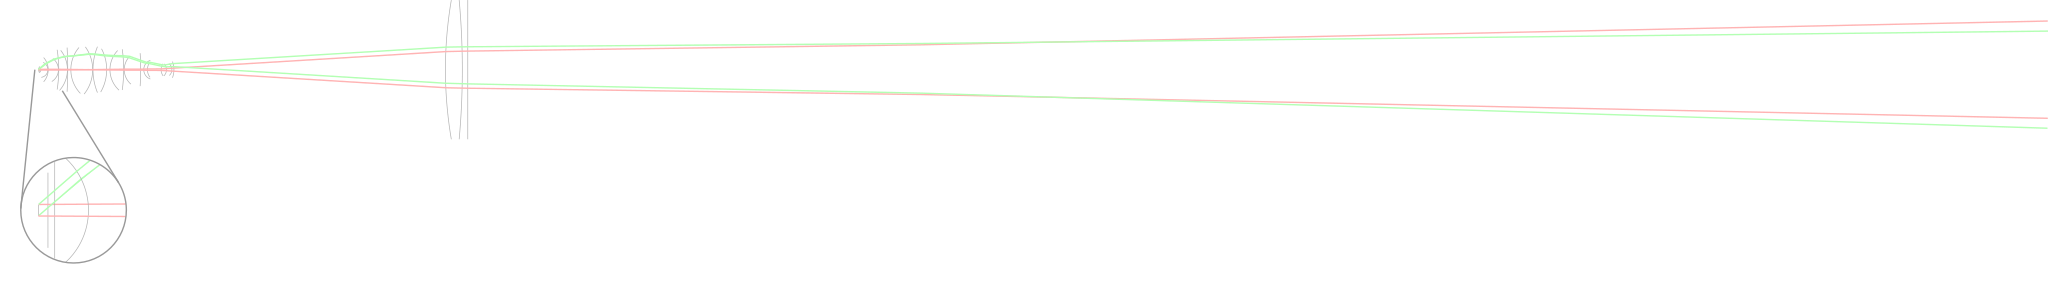
\includegraphics{objective-trace}



  \vspace{-5cm}
  
  \hspace{4cm}\textsf{\Huge Spatio--Angular Microscopy}
  
  \vspace{2cm}
  \hspace{6cm}\textsf{\huge PhD Thesis}


  \vspace{3cm}
  \hspace{4cm}\textsf{\Large Martin Kielhorn}
  
  \vspace{1cm}
  \hspace{4cm}\textsf{\Large July 2012}
\end{titlepage}
\newpage
\include{abstract}
\urlstyle{sf}
%\setcounter{tocdepth}{3}
\section*{Preface}
\begin{flushright}
  M.~K.
\end{flushright}

\noindent
Jena, Germany

\noindent
July 2012

\newpage
\tableofcontents
\printnomenclature
\chapter{Introduction}
\chapter{Methods of controlling illumination patterns}
\chapter{The concept of spatio-angular microscopy}
\label{sec:concept}
\begin{summary}
  Here I introduce the spatio-angular microscope. First I explain the
  concept of its illumination system using exemplary fluorophore
  distributions, that occur in typical specimen.

  Then I describe some decisions we faced during the initial design
  phase concerning the arrangement of optical components. Furthermore,
  I position our method among known approaches of light control for
  microscopy. Of all published techniques for excitation illumination
  control, the light field microscope \citep{Levoy2006} comes closest
  to our approach.  I explain differences between both techniques and
  discuss their respective pros and cons.  I address the peculiarities
  and limitations of the hardware components in chapters
  \ref{sec:dev1} (optics) and \ref{sec:mma} (micromirror based pupil
  plane SLM).  Initially, the details would be detrimental to clarity.

  The effective use of the spatio-angular microscope, requires more
  knowledge about the specimen than a conventional or a SPIM
  microscope \citep{Huisken2004}. Ideally, the distribution of
  refractive index and fluorophores in the specimen should be
  known. If these parameters were precisely known, there would be no
  need for an image in the first place. However, while imaging a known
  specimen, sufficiently good predictions of these parameters can
  often be made. The higher the accuracy of these prognoses, the
  greater the reduction in phototoxicity will be.

  The computer-based selection of appropriate illumination masks
  requires the prediction, or at least an approximate estimation, of
  the three-dimensional distribution of light in the specimen.

  In the last part of this chapter, I describe the computational
  control loop in our spatio-angular
  microscope and touch topics of image processing.
\end{summary}
\section{Motivation}
In order to introduce the basic idea underlying the spatio-angular
microscope, I consider the distribution of excitation light in the
object of a conventional fluorescence microscope:
\figref{fig:hourglass-all}~a) schematically illustrates the side view
of the excitation beam path through objective lens and object in a
confocal microscope. A parallel beam with a circular cross-section
(this cross-section is not shown in the illustration) passes through
the lens. The lens focuses the light in its focal plane.

Between lens and focal plane the light rays form a convergent circular
cone. If refractive index variations in the object are negligible, the
light distribution below the plane of focus forms a cone as well, due
to symmetry.  Assuming a non- or weakly absorbing specimen, the energy
of the light in the circular cross-sections of the cone remains
constant\footnote{The ray-model is valid in large parts of
\figref{fig:hourglass-all}~a), but not everywhere. The Law of
Malus--Lupin states that rays and wavefronts are equivalent as long as
rays do not intersect (caustic), or (FIXME formulas?) a strong
intensity gradient occurs. Thus the ray-model is valid almost
everywhere in the cone, except for a region with a distance of a few
wavelengths to the edge, and the focus itself. While the wave-optical
treatment of these areas is possible, it is computationally much more
expensive than ray tracing. Wave-optical effects either lead to
blurring in a length scale of a few wavelengths or intensity
fluctuations due to interference. If necessary, we can use heuristics
to find an upper bound for the local intensity from ray tracing
results. For this reason we exclusively employ the ray-model in this
work.}\label{sec:ray-valid}.


The fluorescent bead (1), in the focus, would therefore be excited
significantly more than the bead (2) outside the focal plane. Also
shown is the light distribution in the intermediate image plane.

The image of the in-focus bead (1) is sharp, i.e.\ its emanating  % FIXME i need confocal here
fluorescence light is concentrated on an area as small as possible and
positioned exactly on the detection pinhole. Conversely, the image of
the out-of-focus bead (2) is blurred and its fluorescence light is
distributed over a large area.

While only a tiny proportion of the light emitted by the out-of-focus
bead contributes to the detection signal of the confocal
microscope---and therefore hardly affects the image quality, with
respect to overall phototoxicity of the full confocal system---it
would be better to prevent the excitation of the out-of-focus bead in
the first place.

\begin{figure}[!hbt] \centering \svginput{.43}{hourglass-all}
  \caption{{\bf (a)} Two fluorescent beads are illuminated by all
angles that the objective can 
deliver. The sharp image of the in-focus bead is deteriorated by
blurry fluorescence of the out-of-focus bead (2). {\bf (b)} Angular
control allows selective illumination of the in-focus bead (3), and
results in a better image on the camera. {\bf (c)} Angular control,
however, is insufficient, when an extended in-focus area is
illuminated. {\bf (d)} Then, simultaneous spatial and angular control
allows sequential excitation of the in-focus beads, while excluding
the out-of-focus bead (10).}
  \label{fig:hourglass-all}
\end{figure}

The scheme in \figref{fig:hourglass-all}~b) demonstrates how the light
cone would have to be manipulated in order to exclude the out-of-focus
bead (4). The expected fluorescence image in the intermediate image
plane then contains only information from the in-focus bead (3).

Viewed from the in-focus bead (3) the change in illumination
corresponds to a restriction of the light angles. Such control can be
exerted well through a mask in the other focal plane of the objective
lens (also denoted back focal plane or pupil plane).

Thus it is useful and possible to equip a confocal microscope with
angular control. However, in our project we set out to to build a wide
field microscope in order to benefit from the speed and quantum
efficiency of modern cameras.

I now turn to the task of bringing angular control to the wide field
microscope. \figref{fig:hourglass-all}~c) shows a configuration of the
specimen with two in-focus beads (5) and (6), and one out-of-focus
bead (7).  The angular illumination control is ineffective for this
arrangement of beads.  If both in-focus beads, (5) and (6), are
exposed simultaneously, i.e.\ an extended light source illuminates the
entire field, then the out-of-focus bead (7) is always excited.

Only by separate illumination of the in-focus beads (8) and (9), as
shown in \figref{fig:hourglass-all}~d), angular control regains its
function. For this reason a wide field system with angular control,
using a mask in the pupil, requires an additional mask conjugate to
the field.  Therefore, we call our method spatio-angular
microscopy. ``Spatial'' refers to the illumination control in the
field and ``angular'' refers to the control in the pupil plane.

% FIXME 2012 khodjakov schilling

\begin{figure}[!hbt] \centering \svginput{1.5}{memi-simple}
  \caption{Simplified schematic of the illumination system in our
spatio-angular microscope. A homogeneous extended light source
delivers light from the left. It is imaged by lenses $L_1$ and $L_2$
into the intermediate image $F'$. Then the tubelens $L_3$ and the
objective $L_4$ form an image of $F'$ in the sample plane $F$. We use
two spatial light modulators (SLM) to control the spatial and angular
light distribution in the specimen---the focal plane SLM in F', and
the pupil plane SLM in P'.}
  \label{fig:memi-simple}
\end{figure}

\figref{fig:memi-simple} shows the optical path through our prototype
in a simplified form.  From the left side, an extended light source
illuminates the system. A sequence of telecentric lenses $L_1$, $L_2$,
$L_3$ and the objective lens $L_4$ image the light source from F''
into the front focal plane (indicated by F, for field). The etendue
(see page \pageref{sec:etendue} for its definition) of the light
source must be large enough to simultaneously fill both, the pupil P
as well as the field F.

In each of the two planes P' and F' we place a spatial light modulator
(SLM) that allows to control the intensity of the transmitted light.

Looking at the scheme in \figref{fig:memi-simple}, one might argue
that we could save a lens, if we placed the pupil plane SLM into P
instead of P'. There are three reasons why this is neither possible,
nor beneficial: First, the pupil of modern high-performance objective
lenses is typically not accessible. Second, the detection path for
fluorescent light should contain as few optical components as possible
and we can definitely not afford it to be blocked by a SLM.  Third,
the two masks induce non-linear, and therefore difficult to predict,
filtering of spatial frequencies. An analysis requires consideration
of partial spatial coherence, but it should be clear (FIXME) that only
the downstream\footnote{Downstream regarding the propagation direction
  of the excitation light.} SLM will always deliver a good image,
mostly independent of the state of the SLM upstream.

Considering the fact that the image of the focal plane SLM is most
important to us, we decided to place it downstream of the pupil plane
SLM. The focal plane SLM may disturb the image of the pupil plane SLM
in P, but we can always produce very fine, high-contrast structures in
the sample F.

The abiltity to achieve high resolution in the field is the main
difference between our approach and Levoys light field microscope.  In
the light field microscope, the density of the microlenses noticeably
limits the resolution. As opposed to our system, the light field
microscope allows to control the angle of incidence in all field
positions independently.  But, additionally to the reduced focal plane
resolution, this requires a single high-resolution SLM with a
comparatively low refresh rate. We use two small SLMs, which can each
achieve \unit[1]{kHz} frame rate and enable interesting experiments,
e.g.\ optogenetic control of neuron activities.

Furthermore, structured illumination with high resolution patterns
allows us to circumvent the missing cone problem of the widefield
microscope.  Later I will show that depth discrimination improves with
higher resolution patterns (FIXME ref).
\section{An imaging protocol with spatio-angular illumination control}
\subsection{Description of an exemplary biological specimen} 
I now refer to the \celegans\ test sample for phototoxicity that I
introduced in section \ref{sec:intro-phototoxicity}. So far I did not
reach the point of being able to image the development of a real
embryo. Key problems are the low light throughput of the illumination
system and the length of time necessary to update images on the focal
plane display. Nevertheless, I always kept this example in mind while
I was developing the control software for our microscope.

During the first few hours, the embryo develops confined within the
constant volume of its egg, which has an ellipsoidal shape, extends 40
to 60 microns and can be readily observed using a $63\times$ objective
lens. Cell divisions occur every few minutes.  During development the
nuclei get smaller and more dense. In order to track the fate of all
individual cells it is sufficient, to capture one stack per minute
with 41 layers and a $z-$step of 1~micron.
\subsection{Preparation of living embryo samples} 
For an experiment a hermaphrodite worm is cut and the embryos are
placed on an agarose pad, so that they stay immobile during
imaging. This procedure is explained\footnote{Note that
  \cite{Murray2006} describes an improvement of this protocol that
  prevents squeezing the embryos too much.} in \cite{Hope1999}. Of
these embryos, the experimentor chooses a young specimen, that has not
yet divided. We avoid to use fluorescence excitation for this step.
The undivided embryos can be distinguished using the less phototoxic
differential interference contrast (DIC) imaging mode.

\subsection{Sectioning through structured illumination} 
To get an estimate of the initial distribution of the fluorophores in
the embryo I obtain the very first stack with structured illumination
and no angular control. I use this method to avoid the missing cone
problem of the widefield microscope. Perhaps for our particular task
of finding the position of one nucleus within the egg, widefield
images would be just sufficient.  However, for our spatio-angular
method, knowledge about the fluorophore distribution is very important
and therefore we built our microscope such that we can obtain optical
sections.

We compared conventional structured illumination using max$-$min
(FIXME) reconstruction with laser and LED illumination. Although LED
illumination resulted in excellent optical sections, the
reconstruction of laser illuminated images contained artifacts.

% {\color{red} - (FIXME muss das vielleicht in appendix?) In einem
% ersten Entwicklungsschritt, bevor InVision uns den Prototyp fuer das
% spatio-angulare Mikroskop zur Verfuegung stellte, setzten wir einen
% SLM in die Zwischenbildebene. Auf dem SLM wurden vier Streifenmuster
% angezeigt und Wir verglichen einen 70mW 473nm DPSS laser mit 470nm LED
% Beleuchtung (CoolLED).}

Therefore, we decided to implement HiLo (see Appendix FIXME). With
this algorithm, we obtain artifact-free optical sections, regardless
of the illumination source. As another advantage the HiLo method
increases acquisition speed, because only two raw images per slice are
necessary.


% {\color{red} wir haben artefakte in der max-min rekonstruktion
% beobachtet, wenn wir ein grobes streifenmuster (8 forthdd slm pixel
% periode) mit laser beleuchtet haben

%      - irgendwann hat rainer das erklaert aber ich kann mich nicht
% mehr dran erinnern aber es waere cool, wenn ich die story bringen
% koennte
     
% - grobes gitter heisst im amplitudenbild: einige ordnungen (nicht nur
% 3) gehen durch die bfp

%      - irgendwie kam es dadurch im intensitaetsbild zu einigen hoehere
% ordnungstermen

%      - bei LED (extended source) werden die weggemittelt, bei laser
% nicht

%        - ein bisschen kopfzerbrechen bereitet mir noch der bias

%        - im paper habe ich das nicht verstanden [2011 mertz Optically
% sectioned in vivo imaging with speckle illumination HiLo microscopy]

%        - aber ich habe ihr java imagej plugin decompiliert bekommen
% und koennte versuchen ihre implementierung zu verstehen (andererseits
% ist mir das jetzt ziemlich egal)

%        - unter equation 10: The first two terms are variance
% contributions of shot noise. Filtering has the effect of reducing
% noise variance and is taken into account with the integral term. This
% bias must thus be subtracted from $\sigma^2$ prior to the evaluation
% of C. We have also not considered the effects of pixelation in the CCD
% camera. If the pixel size is non-negligible ..  }

\subsection{Computer model for the integration of a priori knowledge
about the biological events} 
Given an initial measurement of the fluorophore distribution of the
embryo, I employ a computational algorithm to find good illumination
conditions for subsequent stack acquisitions. An important requirement
is that the computer can estimate, which areas of the sample should be
protected from illumination.

For our test system, the \celegans\ embryo, it is a promising approach
to represent its three-dimensional fluorophore distribution by a
simple model: Spheres encompassing the nuclei, indicate regions with
fluorophores. When in focus, the spheres are the source of useful,
informative fluorescence signal, but should be protected against
exposure when out of focus.

As I mentioned earlier, there are also unused histones with
fluorophores outside of the nuclei. The images reveal that they occur
in the cytoplasm at a much lower concentration than in the
nuclei. Fluorophores in the cytoplasm have a smaller phototoxic
effect, because any radicals they produce are much less likely to
reach the DNA and therefore inflict substantially less damage.  In the
following my goal is to protect only out-of-focus nuclei from
exposure. The regions in between are used to bring the light in.


During observation, the nuclei, i.e.\ the centers of the spheres, move
slowly within the embryo. For small periods of time we can describe
this movement using a vector field of growth velocities.

A cell division announces itself by a change of the fluorophore
distribution of the nucleus due to chromatin condensation and spindle
formation. Therefore, whenever the computer detects such changes in
the images, in one of the following time steps an additional sphere
should be introduced to account for the new daughter cell.

So far I have implemented a simple algorithm, to convert a time series
of image volumes from a confocal microscope into a sphere model
\citep{Santella2010}.  One of our project partners (Jean-Yves Tinevez,
http://fiji.sc/wiki/index.php/TrackMate) developed a more
sophisticated plug-in for ImageJ, that provides the lineage tree and
snapshots of the developing cells (see \figref{fig:trackmate}).
\begin{figure}[!hbt] \centering
  \pdfinput{6cm}{TrackMate_Celegans_lineage}
  % trim=left bottom right top
  \qquad
  \includegraphics[trim=25cm 0cm 84cm 87cm, clip, height=5cm]{TrackMate_Celegans_lineage_vector}
  \caption{ A detail of a lineage tree visualized in TrackScheme. An
    image of each nucleus is shown in each time step. Note the
    elongated structure of the nucleus before the cell division
    event.}
  \label{fig:trackmate}
\end{figure} Before our microscope can be used for our biological
problem, the computer model has to be extended so that it reliably
tracks the movement of nuclei.  Overlooking any nucleus would prevent
this nucleus from being imaged in later acquisitions and would be a
setback for the experiment.  Estimating the vector field of growth
velocities helps to track nuclei more robustly and allows to predict
their positions for the next exposure.

Currently we have not implemented programs that would fulfill the
requirements for imaging a developing embryo.  However, in the
following text I assume that the described position predictions were
available and I discuss how I determine masks for the focal plane and
pupil plane SLM.

\cite{Murray2006}

TODO FIXME Bernhard Kauslers work is nice
\verb!http://archiv.ub.uni-heidelberg.de/volltextserver/11820/1/thesis_fkaster.pdf!
Live-cell microscopy image analysis for the study of zebrafish embryogenesis
\verb!http://hci.iwr.uni-heidelberg.de/publications/mip/techrep/kausler_12_discrete.pdf!
A Discrete Chain Graph Model for
  3d+t Cell Tracking with High
    Misdetection Robustness

(FIXME read this)


\subsection{Illumination optimization by means of raytracing} 
I now discuss a method to find both SLM masks for image acquisitions
with minimal phototoxicity. First I define a mask for the focal plane
SLM:

From the predicted arrangement of spheres we select in-focus nuclei by
intersecting the model with a planar surface. I then define focal
plane SLM masks to selectively illuminate each of the in-focus nuclei,
by drawing a bright disk in the appropriate position.

Based on such a mask, we can determine which angles can illuminate the
in-focus target nucleus, without exposing out-of-focus nuclei.

As I already explained at the beginning of this chapter on page
\pageref{sec:ray-valid}, ray-optical theory suffices to describe the
light distribution within the sample.

I connect the periphery of an out-of-focus nucleus with a point inside
the in-focus target. This defines a circular cone of rays, that are
propagated through the objective lens. Their intersection with the
pupil plane results in a figure that still very much resembles a
circle---I found that already seven rays lead to good representation
of its perimeter.  An algorithm computes these figures for every
out-of-focus nucleus and for a few in-focus targets points within the
bright areas of the focal plane pattern. In this manner I construct
the desired mask for the pupil plane SLM.

In order to trace the rays into the pupil, I need the design
parameters of the objective lens (vertex position, curvature and
material for all surfaces). Unfortunately, these rarely are publicly
available for high-performance objective lenses. Nevertheless, in
chapter (FIXME) I use a simpler model of the objective lens, that
requires only three parameters: focal length, refractive index of the
immersion medium and numerical aperture. These are always known.

Additionally, I have adapted the model for non-index-matched embedding
of the specimen. This problem occurs when the embryo is illuminated
with an oil immersion objective, using HILO (FIXME ref). It should be
noted, however, that good image quality of the embryo can only be
achieved with an objective lens that has the same immersion index as
the embryo. Otherwise data from 20 microns within the sample will be
severely deteriorated by spherical aberrations.

%\include{app_term}
\bibliographystyle{abbrvnat}
%\bibliography{../state-of-art}
%\bibliography{../All}
\end{document}


%%% Local Variables: 
%%% mode: latex
%%% TeX-master: t
%%% End: 
